\section{Testing Hypothesis and Goodness of Fit}

\subsection{Introduction}

\begin{definition}{\textbf{(Likelihood Ratio)}}
    Consider the two hypothesis to be $H_0$ and $H_1$, we have the following, posterior:
    \begin{equation*}
        P(H_0 | x) = \frac{P(x|H_0)P(H_0)}{P(x)} \qquad P(H_1 | x) = \frac{P(x|H_1)P(H_1)}{P(x)} 
    \end{equation*}    
    The ratio is given as:
    \begin{equation*}
        \frac{P(H_0|x)}{P(H_1|x)} = \frac{P(H_0)}{P(H_1)}\frac{P(x|H_0)}{P(x|H_1)}
    \end{equation*}
    This is the product of the ratio of prior probability and the likelihood ratio. Now, we would like to choose the hypothesis $H_0$ if, we have:
    \begin{equation*}
        \frac{P(H_0|x)}{P(H_1|x)} = \frac{P(H_0)}{P(H_1)}\frac{P(x|H_0)}{P(x|H_1)} > 1 \quad \iff \quad 
        \frac{P(x|H_0)}{P(x|H_1)} > c
    \end{equation*}
    where value of $c$ depends upon your prior probability. 
\end{definition}

\begin{definition}{\textbf{(Neyman-Pearson Paradigm)}}
    One hypothesis is singled out as \emph{null hypothesis} $H_0$ and other as \emph{alternative hypothesis} $H_1$. We have the following terminology as:
    \begin{itemize}
        \item Rejecting $H_0$ when it is true is called \emph{type I error}.
        \item Probability of a type I error is called \emph{significance level} and it is denoted as $\alpha$.
        \item Accepting the null hypothesis when it is false is called \emph{type II error}, and it is denoted by $\beta$. 
        \item The probability that the null hypothesis is rejected when it is false is called \emph{power} of the test, which is equal to $1-\beta$.
        \item The likelihood ratio is called the \emph{test statistics}.
        \item Set of values of the test statistics that leads to rejection of the null hypothesis is called \emph{rejection region}, and set of values that leads to acceptance is called \emph{acceptance region}
        \item The probability distribution of test statistics when the null hypothesis is true is called \emph{null distribution}.
    \end{itemize}
\end{definition}

\begin{definition}{\textbf{(Simple Hypothesis)}}
    If the null and alternative hypothesis each completely specify the probability distribution. This kind of setting is called simple hypothesis. 
\end{definition}

\begin{lemma}{\textbf{(Neyman-Peason)}}
    Suppose that $H_0$ and $H_1$ are simple hypothesis:
    \begin{itemize}
        \item The test that rejects $H_0$ whenever the likelihood ratio is less than $c$ and significance level $\alpha$. 
        \item Then any other test for which significance level is less than or equal to $\alpha$ has power less than or equal to that of the likelihood ratio test. 
    \end{itemize} 
\end{lemma}
\begin{proof}
    Let $p(x)$ denote the pdf or frequency function of the observation. 
    \begin{itemize}
        \item A test of $H_0 : p(x) = p_0(x)$ and $H_1 : p(x) = p_1(x)$ amounts to using a decision function:
        \begin{equation*}
            d(x) = \begin{cases}
                0 & \text{ if } H_0 \text{ is accepted} \\
                1 & \text{ if } H_1 \text{ is rejected} \\
            \end{cases}
        \end{equation*}
        \item Since $d(X)$ is a Bernoulli random varaible, where we have:
        \begin{itemize}
            \item Significance Level: $\mathbb{E}_0[d(X)] = P_0(d(X) = 1)$
            \item Power: $\mathbb{E}_1[d(X)] = P_1(d(X) = 0)$
        \end{itemize}
        \item If we consider the likelihood ratio test as the decision function:
        \begin{equation*}
            d(x) = \begin{cases}
                1 & \text{ if } p_0(X) < cp_1(X) \\
                0 & \text{ otherwise } \\
            \end{cases}
        \end{equation*}
        Please note that $\mathbb{E}_{X\sim p_0(X)}[X] = \alpha$. 
        \item Let $d^*(X)$ be the decision function of another test satisfying $\mathbb{E}_0[d^*(X)] \le \mathbb{E}_0[d^*(x)] = \alpha$. 
        \item Consider the following inequalities:
        \begin{equation*}
            d^*(x)[cp_1(x) - p_0(x)] \le d(x)[cp_1(x) - p_0]
        \end{equation*}
        This follows from the $d(x) = 1$, where $cf_1(x) - f_0(x)> 0$ and if $d(x) = 0$. where $cf_1(x) - f_0(x)\le0$
        \item Integrating the both sides of the inequality above with respected to $x$ as:
        \begin{equation*}
            c \mathbb{E}_1[d^*(X)] - \mathbb{E}_0[d^*(X)] \le c \mathbb{E}_1[d(X)] - \mathbb{E}_0[d(X)]
        \end{equation*}
        and, so we have:
        \begin{equation*}
            \mathbb{E}_0[d(X)] - \mathbb{E}_0[d^*(X)] \le c\brackb{\mathbb{E}_1[d(X)] - \mathbb{E}_1[d^*(X)]}
        \end{equation*}
        Since the LHS of this inequality is non-negative, we have: $\mathbb{E}[d^*(X)] \le \mathbb{E}_A[d(X)]$
    \end{itemize}
\end{proof}

\begin{example}{\textbf{(First Test)}}
    Consider $X_1,\dots,X_n$ be random sample from normal distribution, with unknown mean and variance $\sigma^2$. Given $2$ hypothesis:
    \begin{equation*}
        H_0 : \mu = \mu_0 \qquad H_1 : \mu = \mu_1
    \end{equation*}
    where $\mu_1$ and $\mu_0$ are constant. Consider a significance level of $\alpha$. Then consider likelihood ratio:
    \begin{equation*}
        \frac{f_0(\boldsymbol X)}{f_1(\boldsymbol X)} = \cfrac{\exp\brackb{-\cfrac{1}{2\sigma^2} \sum^n_{i=1}(X_i-\mu_0)^2 }}{\exp\brackb{-\cfrac{1}{2\sigma^2} \sum^n_{i=1}(X_i-\mu_1)^2 }}
    \end{equation*}
    To consider the ratio, we consider the value of $\sum^n_{i=1}(X_i - \mu_1)^2 - \sum^n_{i=1}(X_i - \mu_0)^2$. Expanding the squares:
    \begin{equation*}
        2n\bar{X}(\mu_0 -\mu_1) + n\mu_1^2 - n\mu_0^2
    \end{equation*}
    There are $2$ conditions, so that the likelihood is small:
    \begin{itemize}
        \item If $\mu_0-\mu_1>0$, the likelihood ratio is small if $\bar{X}$ is small. 
        \item If $\mu_0 - \mu_1 < 0$, the likelihood ratio is small if $\bar{X}$ is large. 
    \end{itemize}
    Let's consider the later case. Likelihood-ratio rejects for $\bar{X} > x_0$ for some $x_0$, which we will choose it to give a test of desired level $\alpha$. This means choosing $\mathbb{P}(\bar{X} > x_0) = \alpha$ if $H_0$ is true:
    \begin{equation*}
        \mathbb{P}(\bar{X}>x_0) = \mathbb{P}\bracka{ \frac{\bar{X} - \mu_0}{\sigma/\sqrt{n}} > \frac{x_0 - \mu_0}{\sigma/\sqrt{n}}}
    \end{equation*}
    The null distribution of $\bar{X}$ is a normal distribution with mean $\mu_0$ and variance $\sigma^2/n$, then, we can solve:
    \begin{equation*}
        \frac{x_0 - \mu_0}{\sigma/\sqrt{n}} = z(\alpha)
    \end{equation*}
    for $x_0$ in order to find the rejection region for level $\alpha$ test.
\end{example}

\begin{definition}{\textbf{(P-Value)}}
    As we can see, the testing requires only the null distribution, and we are required to consider the significance level $\alpha$ (which should be $0.01$ and $0.05$). P-value is the smallest significance level at which the null hypothesis would be rejected. 
\end{definition}

\subsection{More Complex Hypothesis Testing}

\begin{definition}{\textbf{(Uniformly Most Powerful)}}
    If the alternative hypothesis $H_1$ is composite, a test is most powerful for every simple alternative in $H_1$ is said to be uniformly most powerful. 
\end{definition}

\begin{example}{\textbf{(2-Sided Test)}}
    Consider $X_1,\dots,X_n$ be random sample from normal distribution, with unknown mean and variance $\sigma^2$. Given $2$ hypothesis:
    \begin{equation*}
        H_0 : \mu = \mu_0 \qquad H_1 : \mu \ne \mu_0
    \end{equation*}
    Please note that in this example, this kind of hypothesis is called two-sided alternative. Consider the test at a specific level $\alpha$ that reject for $\abs{\bar{X} - \mu_0} > x_0$, where $x_0$ is determined such that $\mathbb{P}(\abs{\bar{X} - \mu_0} > x_0) =\alpha$ if $H_0$ is true. We can see that $x_0 = z(\alpha/2)\sigma/\sqrt{n}$:
    \begin{equation*}
    \begin{aligned}
        &\abs{\bar{X}-\mu_0} < \frac{z(\alpha/2)\sigma}{\sqrt{n}}\\
        \iff& \bar{X} - \frac{z(\alpha/2)\sigma}{\sqrt{n}} \le \mu_0 < \bar{X} + \frac{z(\alpha/2)\sigma}{\sqrt{n}} \\
    \end{aligned}
    \end{equation*}
    A $100(1-\alpha)\%$ interval for $\mu$ is give, and so if $\mu_0$ is in the interval, then we accept the null hypothesis. 
\end{example}

\begin{theorem}
    Suppose that for every value $\theta_0$ in $\Theta$ there is a test at level $\alpha$ of the hypothesis $H_0 : \theta = \theta_0$. Denote the acceptance region of the test by $A(\theta_0)$. Then set:
    \begin{equation*}
        C(\boldsymbol X) = \brackc{\theta :\boldsymbol X \in A(\theta)}
    \end{equation*}
    is a $100(1-\alpha)\%$ confidence region for $\theta$. 
\end{theorem}
\begin{remark}
    This means that a $100(1-\alpha)\%$ confidence region for $\theta$ consists of all those values of $\theta_0$ for which the hypothesis that $\theta$ equals $\theta_0$ will not be rejected at level $\alpha$.
\end{remark}
\begin{proof}
    Because $A$ is the acceptance region of a test at level $\alpha$:
    \begin{equation*}
        \mathbb{P}[\boldsymbol X \in A(\theta_0) | \theta = \theta_0] = 1-\alpha 
    \end{equation*}
    Now, we have:
    \begin{equation*}
        \mathbb{P}[\theta_0 \in C(\boldsymbol X) | \theta = \theta_0] = \mathbb{P}[\boldsymbol X \in A(\theta_0) | \theta=\theta_0] = 1-\alpha
    \end{equation*}
    by the definition of $C(\boldsymbol X)$
\end{proof}

\begin{definition}{\textbf{(Generalized Likelihood Ratio Test)}}
    Suppose that the observation: $\boldsymbol X = (X_1,\dots,X_n)$  have a joint density $p(\boldsymbol x | \theta)$:
    \begin{itemize}
        \item Then $H_0$ may specify that $\theta \in \omega_0$ where $\omega_0$ is subset of all possible values of $\theta$
        \item For $H_1$ we consider $\omega_1$ is disjoint from $\omega_0$. 
    \end{itemize}
    Let $\Omega = \omega_0 \cup \omega_1$. The generalized likelihood ratio is $\Lambda^*$ or with the truncated version $\Lambda$ as the small value of $\Lambda^*$ tends to discredit $H_0$: 
    \begin{equation*}
        \Lambda^* = \frac{\max_{\theta\in \omega_0} l(\theta)}{\max_{\theta \in \omega_1}l(\theta)}
        \qquad\Lambda = \frac{\max_{\theta \in \omega_0}l(\theta)}{\max_{\theta \in \Omega}l(\theta)}
    \end{equation*} 
    Note that $\Lambda = \min(\Lambda^*, 1)$. The rejection region is given as $\Lambda \le \lambda_0$, where the threshold $\lambda_0$ is choosen so that 
    \begin{equation*}
        \mathbb{P}(\Lambda \le \lambda_0 | H_0) = \alpha
    \end{equation*}
\end{definition}

\begin{example}{\textbf{(Testing Normal Mean)}}
    Consider $X_1,\dots,X_n$ be random sample from normal distribution, with unknown mean and variance $\sigma^2$. Given $2$ hypothesis:
    \begin{equation*}
        H_0 : \mu = \mu_0 \qquad H_1 : \mu \ne \mu_0
    \end{equation*}
    We have the following specification:
    \begin{equation*}
        \omega_0 = \brackc{\mu_0} \qquad \omega_1 = \brackc{\mu|\mu\ne\mu_0} \qquad \Omega = \brackc{-\infty < \mu < \infty}
    \end{equation*}
    If we maximize over $\omega_0$, as it has only one point, the numerator. For the denominator, we it is clear that the MLE is $\bar{X}$ and so:
    \begin{equation*}
        \max_{\theta \omega_1}l(\theta) = \frac{1}{(2\sigma\pi)^n}\exp\bracka{-\frac{1}{2\sigma^2}\sum^n_{i=1}(X_i - \mu_0)^2} \qquad 
        \max_{\theta \Omega}l(\theta) = \frac{1}{(2\sigma\pi)^n}\exp\bracka{-\frac{1}{2\sigma^2}\sum^n_{i=1}(X_i - \bar{X})^2}
    \end{equation*}
    The ratio is given as:
    \begin{equation*}
    \begin{aligned}
        &\Lambda = \exp\bracka{-\frac{1}{2\sigma^2}\brackb{\sum^n_{i=1}(X_i - \mu_0)^2 - \sum^n_{i=1}(X_i - \bar{X})^2 }} \\
        \iff& \begin{aligned}[t]
            -2\log\Lambda &= \frac{1}{\sigma^2}\bracka{\sum^n_{i=1}(X_i-\mu_0)^2 - \sum^n_{i=1}(X_i-\bar{X})^2}\\
            &= \frac{n(\bar{X} - \mu_0)^2}{\sigma^2}
        \end{aligned}
    \end{aligned}
    \end{equation*}
    Rejecting for small value of $\Lambda$ is equivalent to reject the large value of $-2\log\Lambda$. Together with the identity that $\sum^n_{i=1}(X_i-\mu_0)^2 = \sum^n_{i=1}(X_i - \bar{X})^2 + n(\bar{X} - \mu_0)^2$ . It follows that, under $H_0$:
    \begin{itemize}
        \item $\bar{X} \sim \mathcal{N}(\mu_0, \sigma^2/n)$, which implies that $\sqrt{n}(\bar{X}-\mu_0)/\sigma\sim\mathcal{N}(0, 1)$ 
        \item $-2\log\Lambda\sim\chi^2_1$ is implied from above. 
    \end{itemize}
    We can now construct the rejection region for any significance level to be:
    \begin{equation*}
        \frac{n}{\sigma^2}(\bar{X} - \mu_0)^2 > \chi^2_1(\alpha)
    \end{equation*}
    where $P(Z > \chi^2_1(\alpha)) = \alpha$, recall that we are rejecting the large value of $-2\log \Lambda$. This links back to the original consideration as, we this inequality is equivalent to:
    \begin{equation*}
        \abs{\bar{X}-\mu_0} \ge \frac{\sigma}{\sqrt{n}}z(\alpha/2)
    \end{equation*}
\end{example}

\begin{theorem}
    Under smoothness condition on the probability density, the null distribution of $-2\log\Lambda$ tends to a chi-square distribution with degree of freedom of $\dim\Omega - \dim\omega_0$ as the sample size tends to infinity.
\end{theorem}

\begin{example}{\textbf{(Tests for Multinomial Distribution/Goodness of Fit)}}
    We consider the following testing scenario
    \begin{itemize}
        \item $H_0$: The cell probabilities $p = p(\theta)$ for $\theta \in \omega_0$ (maybe unknown, with dimension of $k$) is constrained on some way.
        \item $H_1$: Cell probabilities are free except the constriants such that they are non-negative and sum to $1$. 
    \end{itemize}
    We have $\Omega$ to be set of $m$ non-negative numbers that sum to one. We have:
    \begin{equation*}
        \max_{p\in\omega_0}\bracka{\frac{n!}{x_1!\cdots x_m!}}p_1(\theta)^{x_1}\cdots p_m(\theta)^{x_m}
    \end{equation*}
    where $x_i$ are observed counts in $m$ cells. We will denote $\hat{\theta}$ as the MLE of $\theta$. For the denominator, with unrestricted MLE, we have $\hat{p}_i = x_i/n$, and so, the ratio is:
    \begin{equation*}
    \begin{aligned}
        &\Lambda = \cfrac{\cfrac{n!}{x_1!\cdots x_m!}p_1(\hat{\theta})^{x_1}\cdot\hat{\theta})^{x_m}}{\cfrac{n!}{x_1!\cdots x_m!}\hat{p}^{x_1}_1\cdots\hat{p}^{x_m}_m} =\prod^m_{i=1}\bracka{\frac{p_i(\hat{\theta})}{\hat{p}_i}}^{x_i} \\
        \implies& \begin{aligned}[t]
            -2\log\Lambda &= -2n\sum^m_{i=1}\hat{p}_i\log\bracka{\frac{p_i(\hat{\theta})}{\hat{p}_i}}
            = 2\sum^m_{i=1}O_i\log\bracka{\frac{O_i}{E_i}}
        \end{aligned}
    \end{aligned}
    \end{equation*}
    As we have $x_i = n\hat{p}_i$, $O_i=n\hat{p}_i$ and $E_i=np_i(\hat{\theta})$. Let's consider the test statistics:
    \begin{itemize}
        \item $\Omega$ allows cell probability to be free (but have to be sum to $1$) so $\dim \Omega = m-1$. 
        \item $p_i(\hat{\theta})$ denpends on $k$-dimensional parameter $\theta$ so $\dim\omega_0 = k$
    \end{itemize}
    The large sample theory, tells us that the distribution of $-2\log\Lambda$ is $\chi^2_{m-k-1}$. 
\end{example}

\begin{definition}{\textbf{(Peason's Chi-Square Statistics)}}
    It is a commonly used to test for goodness of fit, where:
    \begin{equation*}
        X^2 = \sum^m_{i=1}\frac{\brackb{x_i - np_i(\hat{\theta})}^2}{np_i(\hat{\theta})}
    \end{equation*}
\end{definition}

\begin{proposition}
    Peason's statistics and likelihood tests are asymptoticall equivalent under $H_0$
\end{proposition}
\begin{proof}{\emph{(Sketch)}}
    Starting with the value:
    \begin{equation*}
        -2\log\Lambda = 2n\sum^m_{i=1}\hat{p}_i\log\bracka{\frac{\hat{p}_i}{p_i(\hat{\theta})}}
    \end{equation*}
    If $H_0$ is true and $n$ is large, then $\hat{p}_i\approx p_i(\hat{\theta})$. Consider the following Taylor series expansion of:
    \begin{equation*}
    \begin{aligned}
        f(x) &= x\log\bracka{\frac{x}{x_0}} \\
        &= (x-x_0) + \frac{1}{2}(x-x_0)^2\frac{1}{x_0} + \cdots 
    \end{aligned}
    \end{equation*}
    Thus, we have:
    \begin{equation*}
        -2\log\Lambda \approx 2n\sum^m_{i=1}[\hat{p}_i - p_i(\hat{\theta})] + n\sum^m_{i=1}\frac{[\hat{p}_i - p_i(\hat{\theta})]^2}{p_i(\hat{\theta})}
    \end{equation*}
    The first term is zero due to the fact that probabilities sum to $1$, while the second terms is equal to Peason's statistics. Note that Peason's statistics is easier to calculate than the likelihood ratio test.
\end{proof}

\begin{example}{\textbf{(Poisson Dispersion Test)}}
    Gives counts $x_1,\dots,x_n$, we consider:
    \begin{itemize}
        \item $H_0$: The counts are poisson with common parameter $\lambda$. Under $\omega_0$ the MLE of $\lambda$ is $\hat{\lambda} = \bar{X}$. 
        \item $H_1$: The counts have difference rates $\lambda_1,\dots,\lambda_n$. Under $\Omega$ we have $\tilde{\lambda_i} = x_i$ 
    \end{itemize}
    Please note that $\omega_0 \subset\Omega$ is the speical case that they are all equal, so the likelihood ratio is:
    \begin{equation*}
    \begin{aligned}
        &\Lambda = \cfrac{\prod^n_{i=1}\hat{\lambda}^{x_i}\cfrac{\exp(-\hat{\lambda})}{x_i!}}{\prod^n_{i=1}\tilde{\lambda}^{x_i}\cfrac{\exp(-\tilde{\lambda})}{x_i!}} = \prod^n_{i=1}\bracka{\frac{\bar{x}}{x_i}}^{x_i}\exp(x_i-\bar{x}) \\
        \iff&\begin{aligned}[t]
            -2\log\Lambda &= -2\sum^n_{i=1}\brackb{x_i\log\bracka{\frac{\bar{x}}{x_i}} + (x_i - \bar{x})} \\
            &=2\sum^n_{i=1}x_i\log\bracka{\frac{x_i}{\bar{x}}}
        \end{aligned}
    \end{aligned}
    \end{equation*}
    We have the following dimensions for the parameter spaces:
    \begin{itemize}
        \item $\Omega$, there are $n$ independent parameter $\lambda_1,\dots,\lambda_n$ so $\dim\Omega=n$.
        \item $\omega_1$, there is only one parameter so $\dim\omega = 1$
    \end{itemize}
    Thus, the test statistics distribution is $\chi^2_{n-1}$. We can interprete the test statistics as the ratio of $n$ times the estimated variance to estimated mean. 
\end{example}
\begin{remark}
    We can use Taylor series argument to approximate the test statistics for poisson dispersion test:
    \begin{equation*}
        -2\log\Lambda \approx \frac{1}{\bar{x}}\sum^n_{i=1}(x_i - \bar{x})^2
    \end{equation*}
\end{remark}

\subsection{Testing via Plotting}

\begin{definition}{\textbf{(Hanging Rootograms)}}
    Graphical display of the differences between observed and fitted values in historgram. There are multiple sections of rootograms:
    \begin{itemize}
        \item \textbf{Compare Observed Quatities:} We want to compare the observed frequencies with the frequencies fit by the normal distribution. Given the parameters are approximated as $\mu \approx \bar{x}$ and $\sigma \approx \hat{\sigma}$. If $j$-th interval has the left boundary $x_{j-1}$ and right boundary $x_j$. The probability falls in that interval is:
        \begin{equation*}
            \hat{p}_j = \Phi\bracka{\frac{x_j - \bar{x}}{\hat{\sigma}}} - \Phi\bracka{\frac{x_{j-1} - \bar{x}}{\hat{\sigma}}}
        \end{equation*}
        we can predict the count on $j$-th interval as $\hat{n}_j = n\hat{p}_j$, which can be compared to observed counts. Now, we can find the differences between the expected count and observed out. However, we neglet the variability in the estimated expected counts.
        \item \textbf{Variability:} If we neglect the variability in the estimated expected counts as we have:
        \begin{equation*}
            \operatorname{var}(n_j - \hat{n}_j) = \operatorname{var}(n_j) = np_j - np_j^2
        \end{equation*}
        if $p_j$ are small, we have $\operatorname{var}(n_j - \hat{n}_j) \approx np_j$. For a large values of $p_j$ have more varaible differences $n_j - \hat{n}_j$. And, so we expect larger fluctuation in the center than in the tails. 
        \item \textbf{Variance-Stabilizing Transfromation:} Suppose that a random variable $X$ has mean $\mu$ and variance $\sigma^2(\mu)$. If $Y = f(X)$, the method of propagation of error shows that:
        \begin{equation*}
            \operatorname{Var}(Y) \approx \sigma^2(\mu)[f'(\mu)]^2
        \end{equation*}
        If $f$ is chosen so that $\sigma^2(\mu)[f'(\mu)]^2$ is constant, the variance of $Y$ will not depends on $\mu$. Thus the transformation accomplishes variance-stabilizing transformation. 
        \item \textbf{Variability-Stabilizing:} Apply this to the case, and we have:
        \begin{equation*}
            \mathbb{E}[n_j] = np_j = \mu \qquad \operatorname{var}(n_j) \approx np_j = \sigma^2(\mu)
        \end{equation*}
        That is when $\sigma^2(\mu) = \mu$. The variance stabilizing transformation $\mu[f'(\mu)]^2$ should be $f(x) = \sqrt{x }$ does the job so:
        \begin{equation*}
            \mathbb{E}[\sqrt{n_j}] \approx \sqrt{np_j} \qquad \operatorname{var}(\sqrt{n_j}) \approx \frac{1}{4}
        \end{equation*}
        If the method is correct, and so we compare the differences as $\sqrt{n_j} - \sqrt{\hat{n}_j}$. 
        \item \textbf{Interpretation:} We use the deviation of more than $2$ and $3$ standard deviations is large. The run of positive deviations followed by the run of negative deviations and then the large positive deviation in the extreme right tail. This indicates some asymmetry in the distribution. 
        \item \textbf{Hanging Chi-Gram:} The plot of the components of Pearson's chi-square statistics:
        \begin{equation*}
            \frac{n_j - \hat{n}_j}{\sqrt{\hat{n}_j}}
            \implies \operatorname{var}\bracka{\frac{n_j-\hat{n}_j}{\sqrt{\hat{n}_j}}} \approx 1
        \end{equation*}
        Neglecting the variability in the expected counts, $\operatorname{var}(n_j-\hat{n}_j)\approx np_j = \hat{n}_j$, while the it is stabilizes the variance. This leads to the hanging $\chi^2$-gram.
    \end{itemize}
\end{definition}

\begin{definition}{\textbf{(Order Statistics)}}
    Consider the sample of size $n$ from a uniform distribution $[0, 1]$. The ordered sample values by $X_{(1)} < X_{(2)} < \cdots < X_{(n)}$. These values are called order statistics. 
\end{definition}

\begin{remark}{\textbf{(Understanding the Plots)}}
    We can show that:
    \begin{equation*}
        \mathbb{E}[X_{(j)}] = \frac{j}{n+1}
    \end{equation*}
    If the underlying distribution is uniform, the plot is shown in figure below, it is plotted for sample of size $100$ from a uniform distribution. Now, we consider the triangular distribution as we have:
    \begin{equation*}
        f(y) = \begin{cases}
            4y & 0 \le y \le \frac{1}{2} \\
            4-4y & \frac{1}{2} \le y \le 1 
        \end{cases}
    \end{equation*}
    THe ordered observation $Y_{1},\dots,Y_{100}$ are plotted against the points $1/(n+1),\dots,n/(n+1)$:
    \begin{figure}[H]
    \centering
    \begin{subfigure}{.5\textwidth}
        \centering
        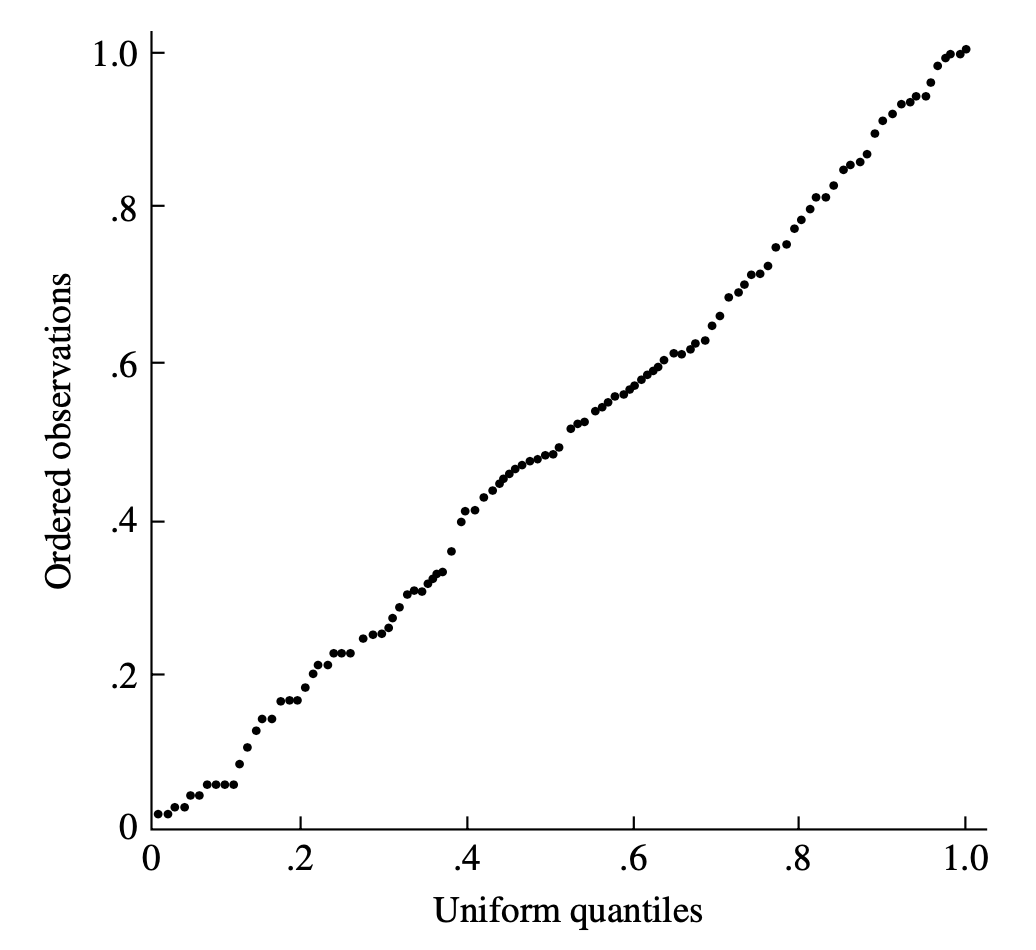
\includegraphics[width=0.7\linewidth]{img/img1.png}
        \caption{Uniform-Uniform Probability Plot}
        \label{fig:1-sub1}
    \end{subfigure}%
    \begin{subfigure}{.5\textwidth}
        \centering
        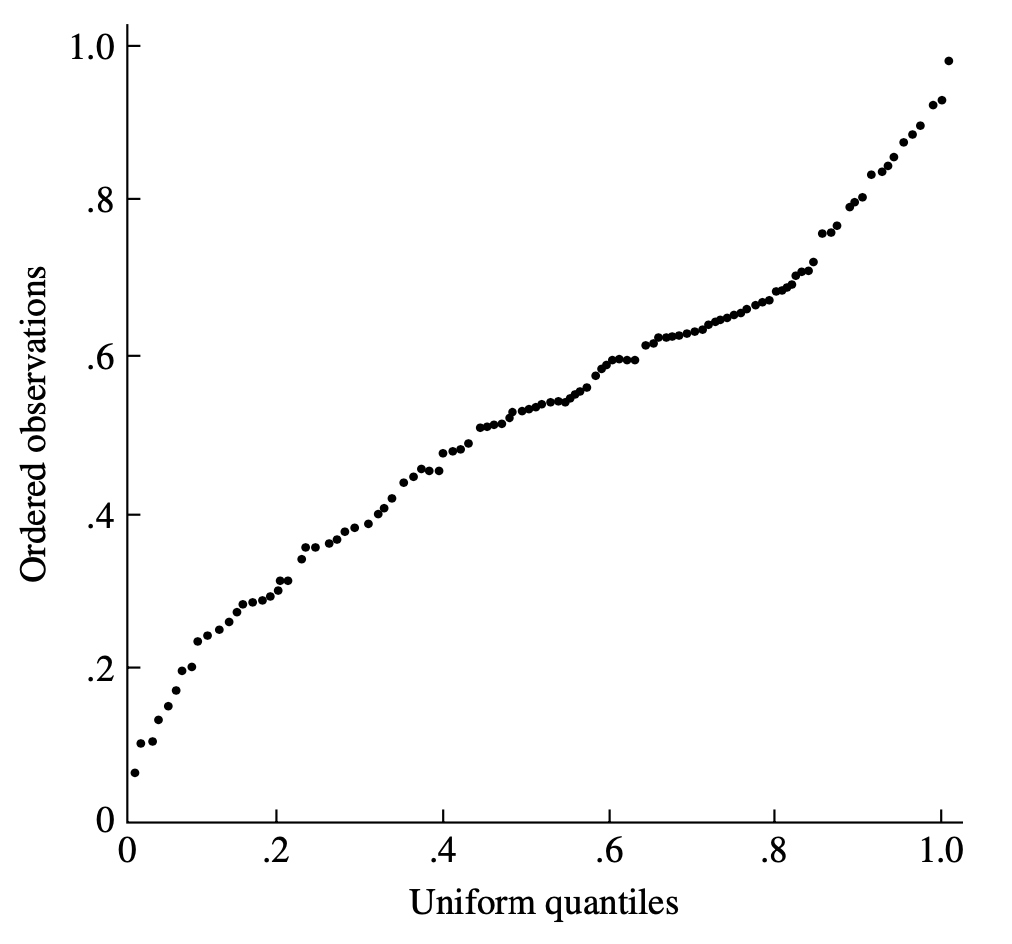
\includegraphics[width=0.7\linewidth]{img/img2.png}
        \caption{Uniform-Triangular Probability Plot}
        \label{fig:1-sub2}
    \end{subfigure}
    \end{figure}
    We can see that there is a clear deviation from the linearity and allow us to describe qualitatively the deviation of the distribution of $Y$'s from the uniform distribution:
    \begin{itemize}
        \item The left tail of the plotted distribution are larger than the expected for a uniform distribution
        \item The right tail is smaller, which tells us that the distribution of $Y$ decreases more quickly than the tails of the uniform distribution. 
    \end{itemize}
\end{remark}

\begin{definition}{\textbf{(Probability Integral Transform)}}
    The technique can be extended to other continuous probability.
    If $X$ is a continuous random variable with a strictly increasing cumulative distribution function, and if $Y = F_X(X)$, then $Y$ has a uniform distribution on $[0, 1]$, as:
    \begin{equation*}
        P(Y \le y) = P(F_X(X) \le y) = P(X \le F^{-1}(y)) = F(F^{-1}(y)) = y
    \end{equation*} 
    This is the uniform of cdf. This transformation is known as probability integral transform.
\end{definition}

\begin{remark}{\textbf{(Probability Plot)}}
    Suppose that it is hypothesized that $X$ follows a certain distribution $F$. Given a sample $X_1,\dots,X_n$, we plot:
    \begin{equation*}
    \begin{aligned}
        F(X_{(k)}) \quad \text{ vs } \quad \frac{k}{n+1} \quad \implies \qquad X_{(k)} \quad\text{ vs }\quad F^{-1}\bracka{\frac{k}{n+1}}
    \end{aligned}
    \end{equation*}
    In some cases, $F$ is of the form $F(X) = G\bracka{\frac{x-\mu}{\sigma}}$, where $\mu$ and $\sigma$ are location and scale parameter. The normal distribution is of this form, we could plot:
    \begin{equation*}
        \frac{X_{(k)} - \mu}{\sigma} \quad \text{ vs }  \quad G^{-1}\bracka{\frac{k}{n+1}}
    \end{equation*}
    or if we plot $X_{(k)}$ vs $G^{-1}\bracka{\frac{k}{n+1}}$. The result would be approixmately a straight line if the model were correct:
    \begin{equation*}
        X_{(k)} \approx \sigma G^{-1}\bracka{\frac{k}{n+1}} + \mu
    \end{equation*}
\end{remark}

\begin{remark}{\textbf{(Slight Modification)}}
    Slight modification of this procedure are sometimes used. For example $\mathbb{E}[X_{(k)}]$ is used instead, as we have:
    \begin{equation*}
        \mathbb{E}[X_{(k)}] \approx F^{-1}\bracka{\frac{k}{n+1}} = \sigma G^{-1}\bracka{\frac{k}{n+1}} + \mu
    \end{equation*}
    The modification yields similar result to the original procedure. 
\end{remark}

\begin{remark}{\textbf{(Another Interpretation)}}
    Recall that $F^{-1}[k/(n+1)]$ is the $k/(n+1)$ quantile of the distribution $F$, the point such that the probability that a random variable with distribution function $F$ is less than it is $k/(n+1)$. We are plotting the ordered observations versus the quantile of the theoretical distribution. 
\end{remark}

\subsection{Testing for Normality}

\begin{definition}{\textbf{(Coefficient of Skewness)}}
    The skewness is usually characterized by the third central moments as:
    \begin{equation*}
        \int^\infty_{i\infty}(x-\mu)^2\varphi(x)\dby x
    \end{equation*}
    which is equal to $0$ given the normal distribution. Now, coefficient of skewness is:
    \begin{equation*}
        b_1 = \frac{1}{ns^3}\sum^n_{i=1}(X_i-\bar{X})^3
    \end{equation*}
\end{definition}

\begin{definition}{\textbf{(Coefficient of Kurtosis)}}
    Symmetric distribution can depart from normality by being heavy tailed or light-tailed. This is characterized by coefficient of Kurtosis as:
    \begin{equation*}
        b_2 = \frac{1}{ns^4}\sum^n_{i=1}(X_i-\bar{X})^4
    \end{equation*}
\end{definition}

\begin{remark}{\textbf{(Test for Normality)}}
    We can use both coefficient for skewness and kurtosis to access the normality of the data. Otherwise, we can use the hypothesis test, but is are difficult to evaluate in closed form but can be approximated by simulation.
\end{remark}

